\documentclass[tikz]{standalone}
\newcommand{\printSQ}[3]{\filldraw [fill=#3, draw=black] (#1-0.5,#2-0.5) rectangle (#1+0.5,#2+0.5);}
\begin{document}
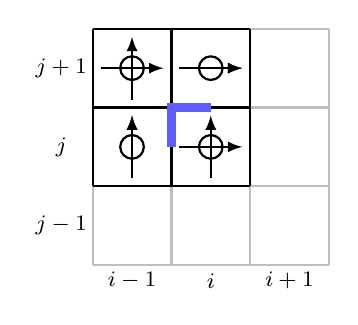
\begin{tikzpicture}[thick,scale=1,line join=round,>=latex]
  \footnotesize
  \foreach \i in {0,1,2,3} {
      \draw [color=lightgray] (0,\i) -- (3,\i);
      \draw [color=lightgray] (\i,0) -- (\i,3);
    }
  \foreach \i in {1,2,3} {
      \draw [color=black] (0,\i) -- (2,\i);
      \draw [color=black] (\i-1,1) -- (\i-1,3);
    }
  \draw [color=blue!63, line width=3] (1.5,2) -- (0.948,2);
  \draw [color=blue!63, line width=3] (1,1.5) -- (1,2.052);
  \foreach \i in {0,1} {
      \foreach \j in {1,2} {
          \draw (\i+0.5,\j+0.5) circle (0.15);
          \ifnum \i < 1 \else \draw [->] (\i+0.1,\j+0.5)--(\i+0.9,\j+0.5); \fi
          \ifnum \j < 2 \else \draw [->] (\i+0.1,\j+0.5)--(\i+0.9,\j+0.5); \fi
          \ifnum \i > 0 \else \draw [->] (\i+0.5,\j+0.1)--(\i+0.5,\j+0.9); \fi
          \ifnum \j > 1 \else \draw [->] (\i+0.5,\j+0.1)--(\i+0.5,\j+0.9); \fi
        }
    }
  
  \draw (0.5,-0.2) node{$i-1$};
  \draw (1.5,-0.2) node{$i$};
  \draw (2.5,-0.2) node{$i+1$};
  \draw (-0.4,0.5) node{$j-1$};
  \draw (-0.4,1.5) node{$j$};
  \draw (-0.4,2.5) node{$j+1$};
\end{tikzpicture}
\end{document}